\newpage
\section{diagramme}
\subsection{Diagramme UML}
\begin{figure}[h]
	\centering
	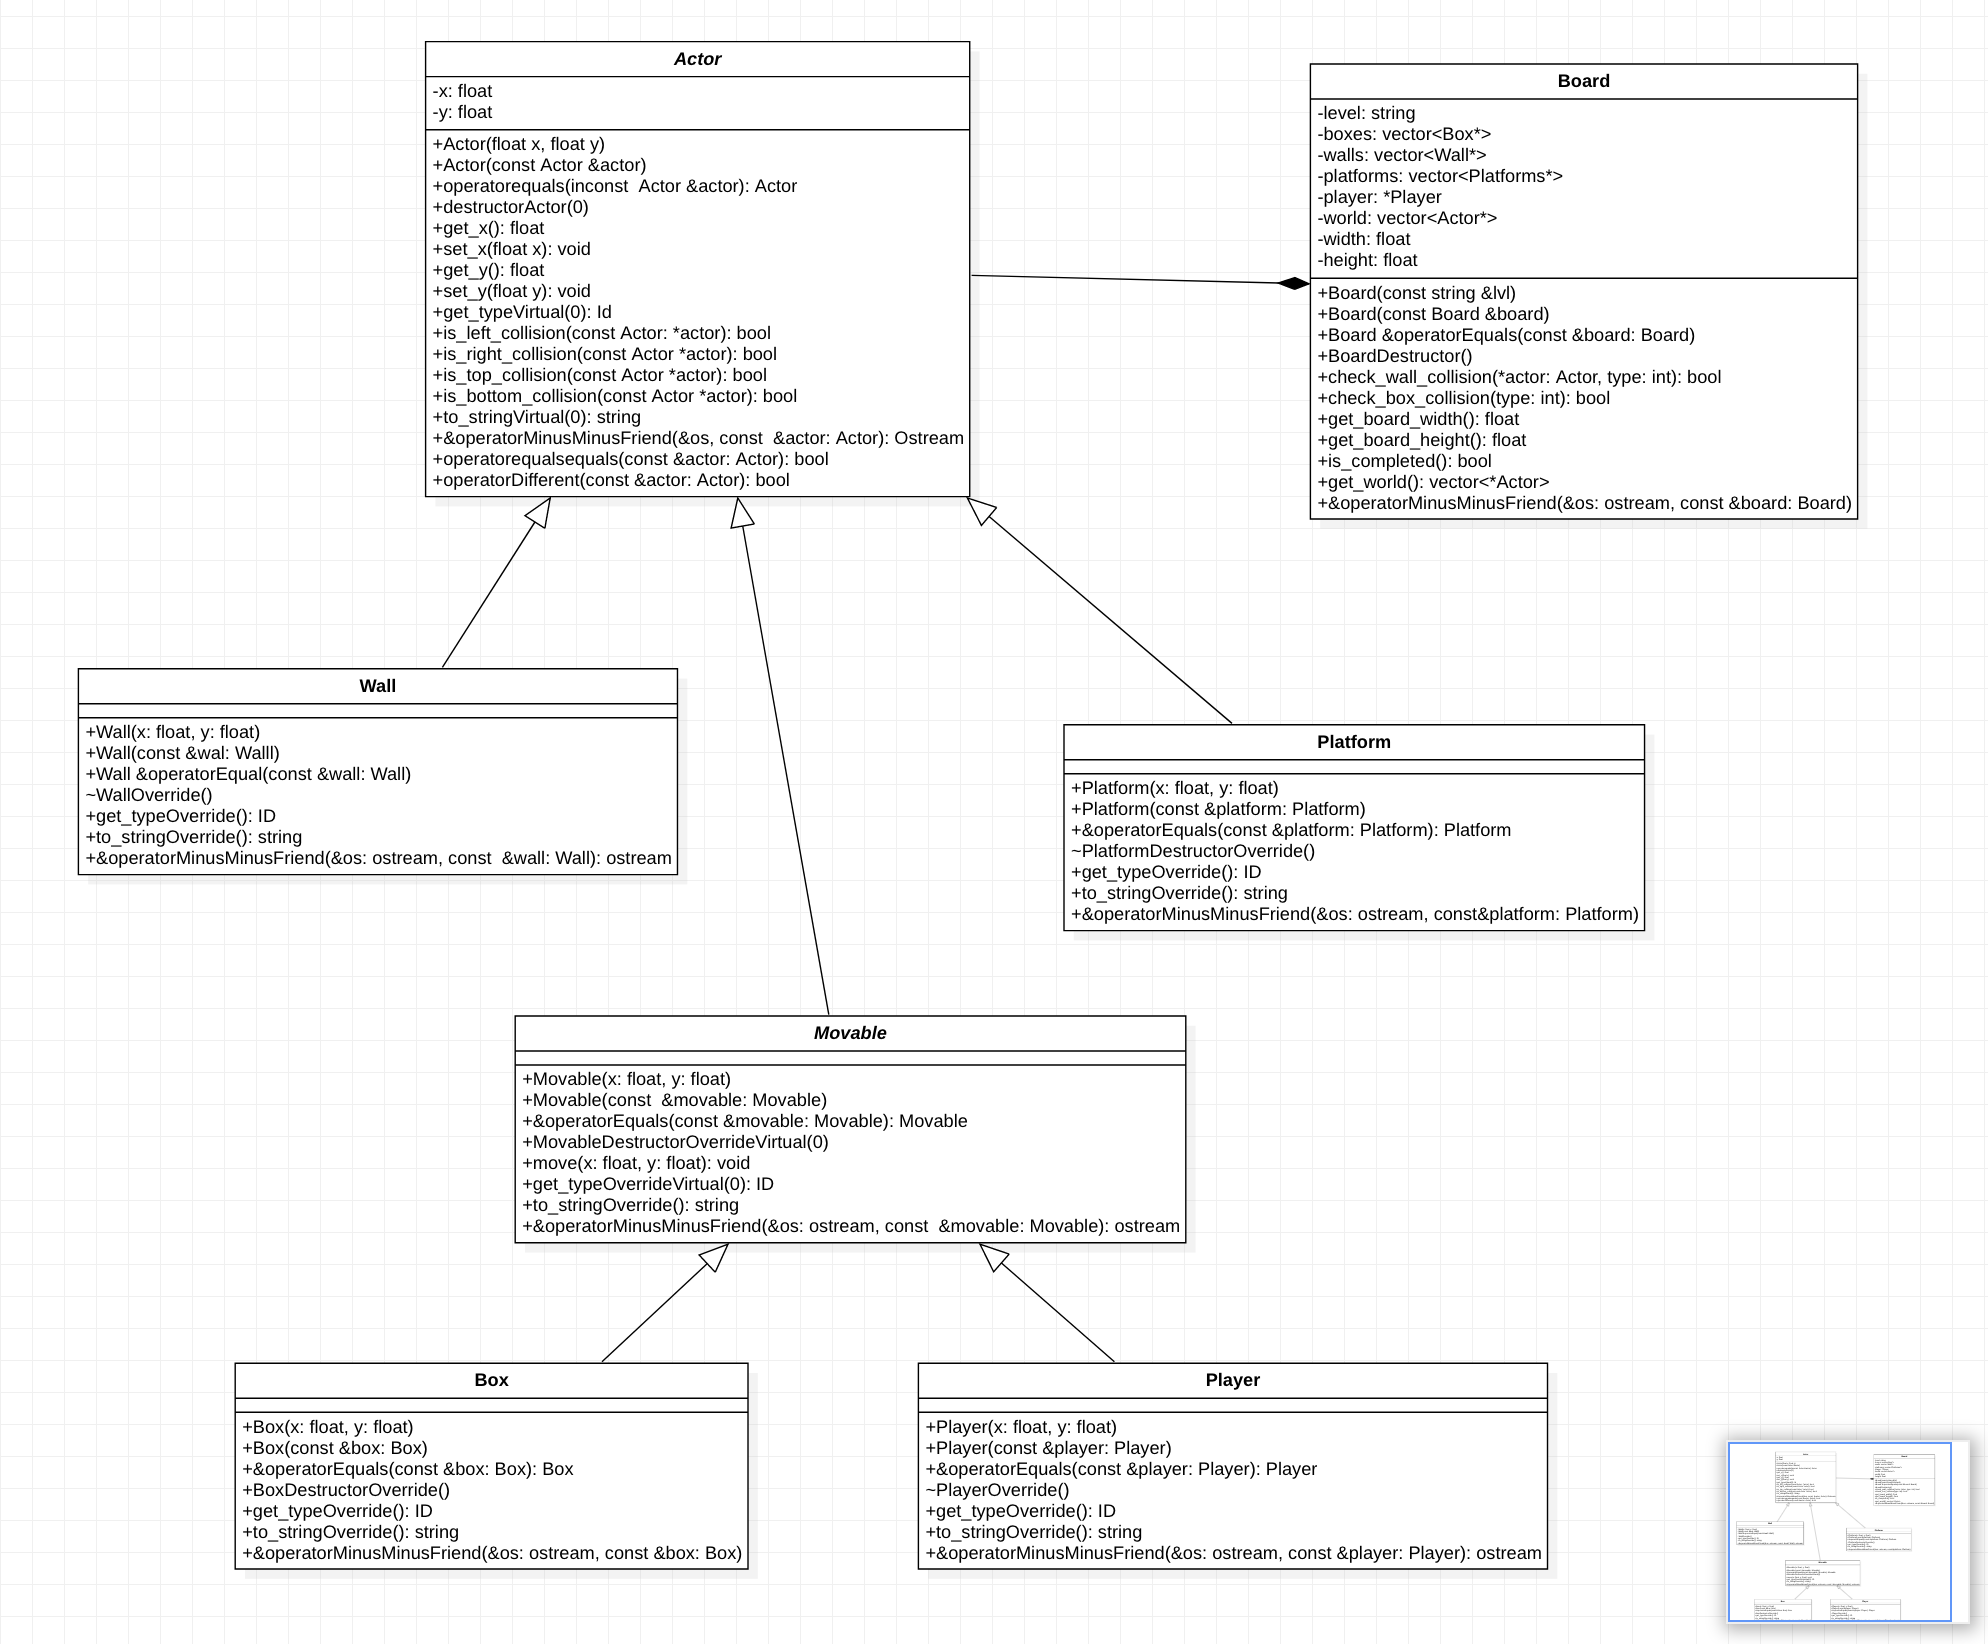
\includegraphics[width=\textwidth] {pictures/uml.png}
	\caption{diagramme de classe}
	\label{fig:UML}
\end{figure}
La Board est composé d'Actor ou de ses spécialisations. Plus précisement, une board est composé d'objet immobile tels que des Walls et des Platforms mais aussi d'objet mobile tels que des Box et un personnage.

\newpage
\subsection{Diagramme d'activité}
\begin{figure}[h]
	\centering
	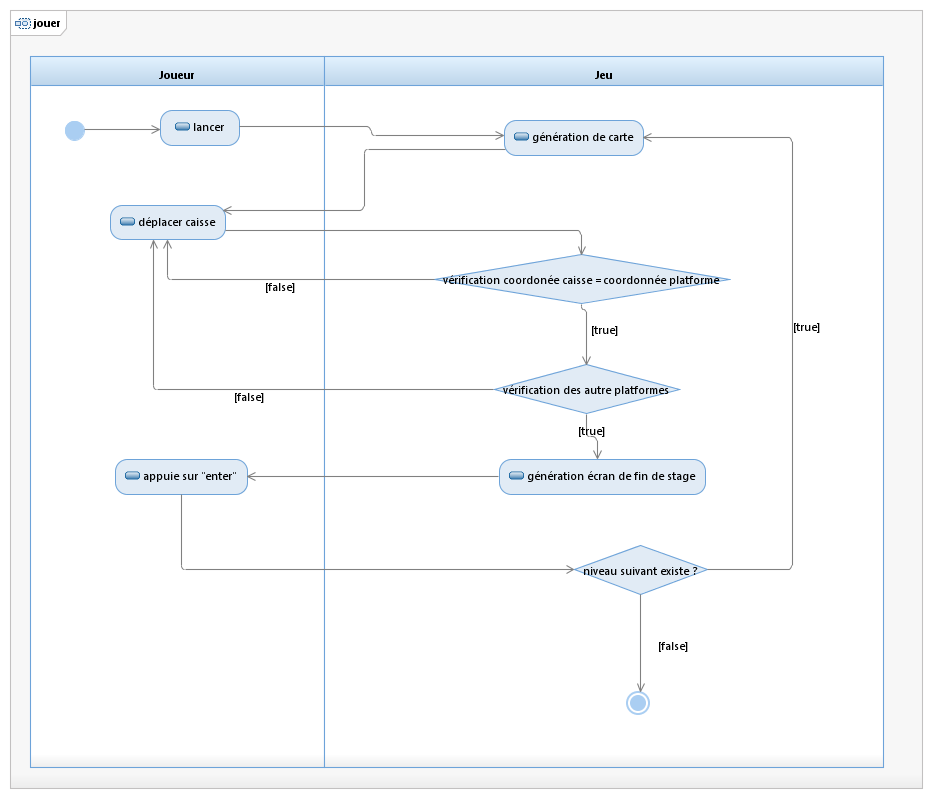
\includegraphics[width=\textwidth] {pictures/dia_activite_jouer.png}
	\caption{diagramme d'activité}
	\label{fig:diagramme_activite}
\end{figure}

\newpage
\subsection{Diagramme Design Pattern State}
\begin{figure}[h]
	\centering
	\includegraphics[width=\textwidth] {pictures/state.png}
	\caption{diagramme du design pattern state}
	\label{fig:diagramme_design_pattern_state}
\end{figure}
Le design pattern state permet de créer des états et de modifier un ou des comportements par rapport à ses états. Dans notre jeu, le state permet d'interchanger entre les différents affichages possibles dans le jeu.